\section{Datenstrukturen}
\label{sec:datastructures}

%% Einführung in die übliche Arbeitsweise bei atomistischen Simulationen

Teilaspekte von Schichtabscheidungen wie Oberflächenreaktionen werden seit vielen Jahren erfolgreich mit KMC- und MD-Methoden simuliert\todo{refs}.
Zur Beschleunigung des Arbeitsablaufes kommt dabei häufig Standardsoftware zum Einsatz, die zwar für allgemeine Systeme optimiert wurde,
im Gegenzug allerdings für spezielle Probleme zu erhöhten Laufzeiten gegenüber spezialisierten Ansätzen führt.
Zu solchen Systemen zählen auch Oberflächenabscheidungen, die aufgrund ihrer geringen Dimensionalität (Oberflächen mit 2 effektiven Dimensionen), langen Laufzeiten (viele Millionen MD-Schritte) und additiver Arbeitsweise (Schrittweises Hinzufügen einzelner Atome) stark von speziellen Optimierungen profitieren können.

%% Vorteile von und Vorgehensweise für Expertensysteme

Die Unterschiede zwischen der Betrachtung allgemeiner und spezieller Systeme liegen dabei in den genutzten Algorithmen und Datenstrukturen:
Bessere Systemkenntnis ermöglicht eine genauere Abschätzung der Häufigkeit bestimmter Operationen, und somit die Wahl und Anpassung von Algorithmen auf die Klasse der zu untersuchenden Systeme.
Dafür werden die Vor- und Nachteile in Form der asymptotischen Laufzeiten von Operationen gegenüber deren Häufigkeit und Speicherverbrauch der Datenstruktur abgewogen.
Als Resultat werden häufige Operationen beschleunigt, wodurch die Effizienz der gesamten Simulation gesteigert und größere Systeme ermöglicht werden.
Es bleibt zu erwähnen, dass der Speicherverbrauch bei den auf das Problem anwendbaren Datenstrukturen linear mit der Systemgröße skaliert, weshalb der primäre Engpass in der Rechenzeit und nicht im Speicherverbrauch liegt.

\subsection{Systemeigenschaften}

Bei den zu betrachtenden Systemen handelt es sich um atomistische Bulks und Oberflächen ohne explizite Simulation der Gasphase.
Für diese ergeben sich folgende Eigenschaften:
\begin{enumerate}
\item Lokalität\\
  Interatomare Einflüsse sind reichweitenbegrenzt
\item Niedriger Diffusionskoeffizient\\
  Atome behalten ihre Nachbarschaft für relativ lange Zeiträume bei
\item Scharfe Oberflächen\\
  Die Oberfläche des Systems ist eindeutig durch eine Menge von Atomen festgelegt
\item Gleichverteilung der Teilchendichte\\
  Es lässt sich eine untere und obere Grenze für Nächstnachbarabstände angeben
\item Teilweise Periodizität\\
  Betrachtete Systeme können entlang ausgewählter Hauptachsen periodisch sein
\end{enumerate}

Einzig das Diffusionskriterium ergibt sich aus der Notwendigkeit, Atompositionen über einen langen Zeitraum ohne Manipulation effizient zu speichern.
Man könnte Diffusionen jedoch auf verschiedene Arten in das Parsivald-Modell einarbeiten.
Dazu zählen explizite MD-Simulationen der Oberfläche ebenso wie Monte-Carlo-Simulationen der Position von Oberflächen- oder Bulkteilchen.
Im Rahmen dieser Arbeit möchte ich zuerst auf diffusionsarme Materialien und Precursorsysteme zurück greifen, bevor der allgemeine Fall betrachtet wird.

Als Resultat der oben genannten Systemeigenschaften lassen sich Annahmen für dir algorithmische Betrachtung des Systemes treffen.
Beispiele solcher Annahmen, die in der Umsetzung des Parsivald-Modelles relevant wurden, zeigt folgende Liste.

\begin{enumerate}
\item Reaktionssimulationen sind auch auf Ausschnitte der Gesamtstruktur durchführbar
\item Nachbarschaftslisten müssen selten aktualisiert werden\\
  Die Reichweite einer Manipulation ist begrenzt
\item Oberflächenatome befinden sich zu einander in direkter Nachbarschaft
\item Die Zahl der Nachbarn unterliegt einer oberen Schranke
\item Divide-and-Conquer-Algorithmen müssen aufwendigeres Stitching betreiben
\end{enumerate}

Ohne diese Annahmen stellten einige der ausgewählten Operationen das System nur unzureichend dar.

\subsection{Benutzte Operationen}

\begin{table}[b]
  \caption[datasymbols]{Symbole für Laufzeit- und Speicherabschätzungen}
  \label{tab:datasymbols}
  \begin{tabularx}{\textwidth}{|lX|lX|}
    \hline
    {Symbol} & {Bedeutung} & {Symbol} & {Bedeutung} \\
    \hline
    \BigO{expr} & Worst-Case-Komplexität & $n$ & Zahl der Atome \\
    $k$ & Zahl von Nächstnachbarn & $b$ & Zahl der Bins \\
    $k_r$ & Zahl von Nachbarn mit $d \leq r_c$ & $r_c$ & Cutoff-Radius \\
    $r_s$ & Suchradius & $s$ & lineare Raumgröße \\
    \hline
  \end{tabularx}
\end{table}

\todo[inline]{Referenzen der optimalen Laufzeiten!}

Aus Sicht der aufrufenden Simulation ist die Wahl der unterliegenden Datenstruktur nicht ersichtlich.
Für sie besteht die Interaktion aus Operationen, die auf die Menge von Atomen ausgeführt werden.
Das beinhaltet Konstruktions-, Manipulations- und Suchoperationen auf dieser Menge.
Ein Vergleich der asymptotischen Laufzeiten ist in Tabelle \ref{tab:dataruntimes} dargestellt.

\subsubsection{Konstruktion}
Damit wird der einmalige Aufbau der gesamten Struktur aus einer beliebigen Menge von Atomen bezeichnet.
Dadurch steht die eigentliche Laufzeit dieser Operation im Hintergrund.

Liegt kein separater Algorithmus vor, kann die Struktur durch iterative Einfügung einzelner Atome angenähert werden, und verhält sich somit linear zur Laufzeit der Einfügungsoperation, und somit maximal quadratisch zur Zahl der Atome.
Optimal ist hier \BigO{n} bei simplen Listen, im Gegensatz zu \BigO{n^2} bei Nachbarschaftslisten\ref{}.

\subsubsection{Einfügung}
Je nach Datenstruktur auch Push-Operation genannt, bezeichnet sie das Einfügen eines neuen Atomes in eine bestehende Struktur.
Dies geschieht im Parsivald-Modell nach erfolgreichen Reaktionen von Gasmolekülen auf der Oberfläche, bei denen die neu aufgebrachten Atome dem Simulationsraum beigefügt werden.
Da diese Operation vergleichsweise häufig aufgerufen wird, bieten sich Strukturen an, bei denen nur die lokale Nachbarschaft, nicht aber die gesamte Struktur aktualisiert werden muss.

Optimale Laufzeit ist das Hinzufügen eines Atomes an das Ende einer Liste in konstanter Zeit (\BigO{1}), jedoch verlangen einige Strukturen den Vergleich mit allen anderen Atomen, wodurch sich \BigO{n} ergibt.

\subsubsection{Modifikation}
Auch als Up\-date-Operation bekannt, führt sie eine Aktualisierung der Positionen oder des Typen\footnote{Einige Anwendungen erfordern die separate Betrachtung verschiedener Adsorptions- oder Oxidationszustände durch separate Atomtypen} einzelner oder mehrerer Atome durch.

Auch hier lässt sich konstante Zeit als Optimum angeben, wo hingegen beispielsweise Nachbarschaftslisten komplett neu aufgebaut und somit Laufzeitgrenzen von \BigO{n} angegeben werden müssen.

\subsubsection{Entfernung}
Als Gegenstück zur Push-Operation entfernt diese eines oder mehrere Atome aus dem Simulationsraum.
Diese Operation wird angewandt, wenn durch Reaktionen einzelne Liganden von der Oberfläche entfernt werden und findet somit Anwendung bei Simulationen, die den gesamten Precursor betrachten.
Es gelten die gleichen Laufzeitgrenzen wie bei der Einfügung von Atomen.

\subsubsection{Nachbarschaftssuche}
Ihrem Namen entsprechend sucht diese Operation nach allen Atomen in der Nachbarschaft eines vorher bekannten Atomes.
Sie wird beim Parsivald-Modell genutzt, um die lokale Nachbarschaft eines Referenzatomes für eine MD-Simulationen zu extrahieren, und somit bei jedem ausgewählten KMC-Ereignis ausgeführt.

Die Laufzeit variiert stark zwischen \BigO{1} für Nachbarschaftslisten, die die Komplexität in die anderen Operationen auslagern, und \BigO{n}, falls die Position aller Atome explizit verglichen werden muss.
Häufig ist die Laufzeit auch proportional zur oberen Grenze der Zahl von Nachbarschaftsatomen und somit zum kubischen Suchradius.

\subsubsection{Ortssuche}
Im Unterschied zur Nachbarschaftssuche sucht man hier alle Atome im Umkreis eines beliebigen Punktes im Raum.
Diese Operation wird zur Identifizierung eines Reaktionsortes und somit zum Aufbau eines KMC-Ereignisses genutzt.
Damit ist sie die häufigste Operationen und sollte im Mittelpunkt von Optimierungsbemühungen stehen.
Da beide Nachbarschaftssuchen in einander überführbar sind, ist ihre Komplexität mit wenigen Ausnahmen gleich.

\subsubsection{Oberflächensuche}
Diese Operation sucht die Oberfläche, entweder entlang einer definierten Geraden oder im Umkreis eines Punktes.
Die Art der Eingangsgröße kann von der aufrufenden Simulation zugunsten der Laufzeit gewählt werden.


\begin{table}
  \centering
  \begin{tabularx}{\textwidth}{X|*8c}
    Datenstr.  &  Konstr.          &  Einfüg.          &  Modif            &  Entf.            &  Ortss.                &  NB-Su.               &  Oberfl.         &  RAM                          \\
    \hline
    Atomliste  &  \cG{$n$}         &  \cG{$1$}         &  \cG{$1$}         &  \cG{$1$}         &  \cR{$n$}              &  \cR{$n$}             &  \cR{$n$}        &  \cG{$n$}                     \\
    NB-Listen  &  \cY{$n\log{n}$}  &  \cR{$n$}         &  \cR{$n$}         &  \cR{$n$}         &  \cR{$n$}              &  \cG{$1$}             &  \cR{$n$}        &  \cR{$\frac{r_c^3}{s^3}n^2$}  \\
    Binning    &  \cG{$n$}         &  \cG{$1$}         &  \cG{$1$}         &  \cG{$1$}         &  \cG{$r_s^3$}          &  \cG{$r_s^3$}         &  \cR{$c$}        &  \cY{$n+c$}                   \\
    Octree     &  \cY{$n\log{c}$}  &  \cY{$\log{c}$}   &  \cY{$\log{c}$}   &  \cG{$1$}         &  \cY{$r_s^3\log{c}$}   &  \cY{$r_s^3\log{c}$}  &  \cY{$\log{c}$}  &  \cY{$n+c^\frac{2}{3}$}       \\
    k-d-Baum   &  \cY{$n\log{n}$}  &  \cY{$\log{n}$}   &  \cY{$\log{n}$}   &  \cY{$\log{n}$}   &  \cY{$r_s^3\log{n}$}   &  \cY{$r_s^3\log{n}$}  &  \cY{$\log{n}$}  &  \cG{$n$}                     \\
    Delaunay   &  \cY{$n\log{n}$}  &  \cY{$k\log{k}$}  &  \cY{$k\log{k}$}  &  \cY{$k\log{k}$}  &  \cG{$r_s^3+\log{n}$}  &  \cG{$r_s^3$}         &  \cG{$1$}        &  \cY{$nk$}                    \\
    \hline
    %Atomfeld  &  \cG{$n$}         &  \cG{$1$}         &  \cG{$1$}         &  \cG{$1$}         &  \cR{$n$}              &  \cR{$n$}             &  \cR{$n$}        &  \cG{$n$}                     \\
  \end{tabularx}
  \vspace{1em}
  \begin{tabularx}{0.7\textwidth}{*3C}
    \cG{optimal} & \cY{annehmbar} & \cR{Bottleneck} \\
  \end{tabularx}
  \label{tab:dataruntimes}
  \caption[Laufzeitabschätzung genutzter Operationen auf verschiedenen Datenstrukturen]{
    Abschätzung des Speicheraufwands und der asymptotischen Laufzeit ausgewählter Operationen auf verschiedenen Datenstrukturen
    \\
  }
\end{table}

\subsection{Klassen von Datenstrukturen}

Die Vielzahl der verfügbaren Datenstrukturen und Algorithmen lassen sich in generelle Kategorien nach ihrer Arbeitsweise einordnen.
Diese teilen ihre Funktionsweise, so dass Algorithmen innerhalb der Klasse oftmals austauschbar sind.

\subsubsection{Listen}

Listen sind die einfachste Datenstruktur zur Behandlung von Punktwolken.
Die einzelnen Atome werden in einer Liste gespeichert, wodurch Manipulationsoperationen in optimaler konstanter Zeit möglich sind, Nachbarschaftsoperationen andererseits Vergleiche mit sämtlichen Atomen anstellen müssen, wodurch die Laufzeit der zeitkritischen Operationen die Worst-Case-Laufzeit von \BigO{n} annimmt.

\subsubsection{Nachbarschaftslisten}

Nachbarschaftslisten sind Atomlisten, die für jedes Atom eine Referenz zu allen Atomen innerhalb einer begrenzten Nachbarschaft beinhalten.
Diese Referenzen müssen bei jeder Manipulation aufwendig aktualisiert werden, wodurch im Gegenzug die Nachbarschaftssuche in konstanter Zeit (\BigO{1}) beziehungsweise je bei weiteren Anforderungen mit \BigO{r} skalieren.
Nachbarschaftslisten verringern in MD-Simulationen mit Kraftfeldern mit begrenzter Reichweite die Programmlaufzeit signifikant, bei häufigen Aktualisierungen bietet sich jedoch auch Binning an.

Der Vollständigkeit halber möchte ich erwähnen, dass einige der \BigO{n}-Operationen durch clevere Optimierung und Suche innerhalb der direkten Nachbarschaft beispielsweise auf \BigO{rk} reduziert werden kann.
Bei großen Verschiebungen der Atomposition muss dafür zuvor einer der Nachbarn gesucht werden, wodurch sich erneut eine \BigO{n}-Operation vorschiebt und die asymptotische Laufzeit wieder auf \BigO{n} erhöht wird.

\subsubsection{Binning}

Eine implizite Möglichkeit, die lokale Nachbarschaft zu referenzieren, findet man in Binning.
Dafür zerlegt man den Raum in kleinere Quader, in denen man die enthaltenen Atome referenziert.
Die Nachbarn ergeben sich dann aus einer Suche innerhalb der benachbarten Quader.
Notwendig ist eine eindeutige Addressierung der Quader aus der Atomposition sowie die Suche der benachbarten Quader, die auch bei periodischen Simulationsräumen eindeutig ist.

\subsubsection{Suchbäume}

Eine andere Möglichkeit, Bäume für die Optimierung von Suchfunktionen zu nutzen, findet sich in k-dimensionalen Bäumen, auch k-d-Trees genannt.
Diese sind eine rekursive Datenstruktur, die alle Atome entlang einer Hauptachse sortieren, das Median-Element als Root-Knoten herausnehmen und jeweils aus der linken und rechten Seite einen neuen k-d-Baum aufbauen.
Nicht ganz offensichtlich ist damit jede Nachbarschafts- und Ortssuche in \BigO{N_r\log{n}} möglich.\todo{N - Obere Schranke der Zahl der Nachbarn innerhalb des Suchradius}{}
Dies geht auf Kosten der Manipulationsoperationen, die in \BigO{\log{n}} laufen.

\subsubsection{Triangulationen}

Triangulationen kann man als eine spezielle Form von Nachbarschaftslisten betrachten.
Sie teilen den gesamten Raum in nicht-überschneidende k-Simplexe, deren Ecken auf vordefinierten Punkten liegen.
Damit teilen sich alle Atome mindestens einen Simplex mit ihrem nächsten Nachbarn, jedoch nicht notwendigerweise mit allen Nachbarn innerhalb eines bestimmten Radius'.
Triangulationen werden in verschiedenen Varianten genutzt, wobei in dieser Arbeit die populäre Delaunay-Triangulation aufgrund ihrer Dualität zu Voronoi-Diagrammen und der direkten Verbindung zu Alpha-Formen betrachtet wird.

\begin{figure}[bhpt]
  \captionsetup[subfigure]{singlelinecheck=false}{
    \def\subfigwidth{0.23\textwidth}
    \def\svgwidth{\textwidth}
    \begin{subfigure}[t]{\subfigwidth}
      \includegraphics[width=\textwidth]{datastructures-a}
      \subcaption{Ohne Binning}
      \label{fig:datastructures-a}
    \end{subfigure}
    \hfill
    \begin{subfigure}[t]{\subfigwidth}
      \includegraphics[width=\textwidth]{datastructures-b}
      \subcaption{k-d-Arrays}
      \label{fig:datastructures-a}
    \end{subfigure}
    \hfill
    \begin{subfigure}[t]{\subfigwidth}
      \includegraphics[width=\textwidth]{datastructures-c}
      \subcaption{Octree}
      \label{fig:datastructures-a}
    \end{subfigure}
    \hfill
    \begin{subfigure}[t]{\subfigwidth}
      \includegraphics[width=\textwidth]{datastructures-d}
      \subcaption{k-d-Baum}
      \label{fig:datastructures-a}
    \end{subfigure}
  }
  \caption[Übersicht über räumliche Datenstrukturen]{Übersicht über räumliche Datenstrukturen}
  \label{fig:datastructures}
\end{figure}

\subsection{\todo{rename}{Berücksichtigte Datenstrukturen}}

\subsubsection{Octree-Binning}
Octree-Binning ist eine mögliche Optimierung der Binning-Methode, bei der man zur Aufteilung des Raumes nicht auf k-dimensionale Arrays, sondern auf einen sogenannten Octree zurück greift.
Als diesen bezeichnet man eine dreidimensionale Struktur, die eine Zelle rekursiv in je 8 gleichartige Zellen halber Breite aufteilt, bis man eine gewünschten Zellgröße erreicht.
Durch Bitoperationen lassen sich die Zellen effizient und identisch zu k-d-Arrays addressieren, jedoch ist jede Zelladdressierung auf dem Baum mit einer \BigO{\log{c}}-Operation verbunden.
Der Hauptunterschied findet sich jedoch in der Oberflächen- und Ortssuche:
8 benachbarte, leere Zellen können effektiv zu einer Superzelle zusammen gefasst werden, die bei Suchoperationen gemeinsam übersprungen werden.
Somit reduziert sich die Speicherkomplexität von großen dreidimensionalen Dünnschichtsystemen auf die Komplexität eines zweidimensionalen Systemes, auf Kosten zusätzlicher Buchhaltung mit \BigO{\log{c}}-Komplexität.


\begin{algorithm}
  \begin{algorithmic}
    \Input $atoms$ - Liste von Atomen
    \Input $size[3]$ - Größe des Simulationsraumes
    \Input $depth$ - Tiefe des Octrees. Legt die Zellgröße fest
    \Assumption Alle Atome befinden sich im Simulationsraum
    \Result Stammzelle eines Octrees, der alle Atome enthält
    \State
    \Function{construct-octree}{$atoms, size, depth$}
    \State $cellsize[0] \gets size[0]\cdot2^{-depth}$
    \State $cellsize[1] \gets size[1]\cdot2^{-depth}$
    \State $cellsize[2] \gets size[2]\cdot2^{-depth}$
    \State $root \gets$ new Octree($depth$)
    \ForAll{$atom$ in $atoms$}
    \State $cellindex[0] \gets \lfloor atom.pos[0] / cellsize[0] \rfloor$
    \State $cellindex[1] \gets \lfloor atom.pos[1] / cellsize[1] \rfloor$
    \State $cellindex[2] \gets \lfloor atom.pos[2] / cellsize[2] \rfloor$
    \State $cell \gets$ \Call{getcell-octree}{$root, cellindex$, true}
    \State \Call{addatom}{cell, atom}
    \EndFor
    \State \Return $root$
    \EndFunction
  \end{algorithmic}
  \label{alco:octree-construction}
  \caption[Octree-Konstruktion]{Octree-Konstruktion: Es handelt sich um einen typischen Binning-Algorithmus, dessen Octree-Eigenschaften in der Funktion \Call{getcell-octree}{} liegen.}
\end{algorithm}

\begin{figure}[tbhp]
  \centering
  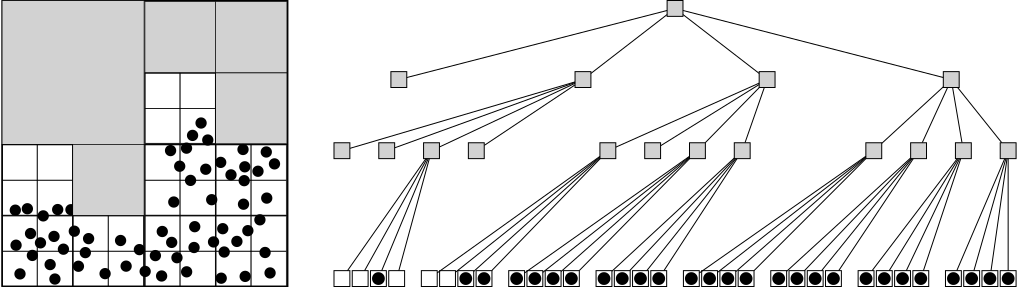
\includegraphics[width=\textwidth]{octree}
  \label{fig:octree}
  \caption[Quadtree-Veranschaulichung eines Octrees]{Quadtree (2d) zur Veranschaulichung der Funktionsweise eines Octrees (3d):\\
    Rekursive Unterteilung der interessanten Zellen bis zur gewünschten Auflösung, dann zellweises Binning.
    Dabei werden nur benutzte Zellen dynamisch allokiert, wodurch sich bei Oberflächensystemen Einsparungen in Speicherverbrauch und Laufzeit ergeben.
  }
\end{figure}

\begin{algorithm}
  \begin{algorithmic}
    \Input $root$ - Stammzelle des Octrees
    \Input $index[3]$ - globale Adresse der Zielzelle
    \Input $allocate$ - Ob die Zelle neu erstellt werden soll
    \Result null falls leer, sonst Zielzelle
    \State
    \Function{getcell-octree}{root, index, allocate}
    \State $depth \gets $\Call{depth}{root}
    \Comment{Tiefe, an der sich die Zielzellen befinden}
    \State $cell \gets root$
    \While{$depth > 0$}
    \If{not $cell.children$}
    \If{allocate}
    \State $cell.children \gets $new cell[8]
    \Else
    \State \Return null
    \EndIf
    \EndIf
    \State $depth \gets depth-1$
    \State $childid \gets $\Call{bitand}{index[0], $2^{depth}$}
    \State $childid \gets childid+2\cdot$\Call{bitand}{index[1], $2^{depth}$}
    \State $childid \gets childid+4\cdot$\Call{bitand}{index[2], $2^{depth}$}
    \State \Comment{Indiziert die Subzelle aus der globalen Position}
    \State $cell \gets cell.children[childid]$
    \EndWhile
    \State\Return cell
    \EndFunction
  \end{algorithmic}
  \caption[Zell-Addressierung in Octrees]{Zell-Addressierung und -Allokierung im Octree: Bei jedem Schritt wird der Raum in 2 Unterzellen je Raumdimension geteilt, woraus eine Laufzeit von \BigO{\log{depth}} resultiert}
  \label{algo:octree-adressing}
\end{algorithm}

Weitere Laufzeitoptimierungen ergeben sich bei Betrachtung der Addresszugriffe.
So wird bei der Ereignissuche wiederholt auf Zellen in direkter Nachbarschaft zugegriffen.
Durch Access Caching speichert man den letzten Zellzugriff und sucht bei weiteren Zugriffen auf dem Octree in der Nachbarschaft dieser Zelle, statt jede Zelladdressierung beim Root-Knoten zu beginnen.
Bei Aufruf einer leeren, nicht-allokierten Zelle speichert man stattdessen deren kleinste Superzelle, wodurch man automatisch die kleinste Superzelle der Nachbarschaft referenziert und folgende Suchoperationen signifikant verkürzt.
Addressierung der kleinsten gemeinsamen Superzelle geschieht durch Vergleich des höchsten unterschiedlichen Bits der Addresse, der auf einigen Prozessorarchitekturen fest im Chipsatz verankert ist und somit in konstanter Zeit läuft.

\todo[inline]{Wars das? Formeln?}

\subsection{k-d-Baum}

Recherchiert man optimale Strukturen für Suchoperationen, stößt man schnell auf k-dimensionale Bäume, oder kurz k-d-Bäume.
Diese unterteilen einen kartesischen Raum in orthogonale Zellen, die jeweils genau ein Atom beinhalten, welches jedoch auf einer der Zellgrenzen liegt.
Durch Algorithmus \ref{algo:kdtree-construction} zur Konstruktion eines k-d-Baumes ergibt sich ein balancierter Baum mit Atomen als Knoten, der als besondere Eigenschaft radiale Suchen nach beliebigen Punkten beschleunigt.
Ist ein Knoten weiter entfernt als eine vorherige Referenz, so sind dessen Kinder ebenfalls weiter entfernt.
Somit lässt sich per impliziter binärer Suche jedes nächste Atom in \BigO{\log{n}} finden.
In Verbindung mit einem Heap lässt sich auch eine feste Anzahl von Atomen in \BigO{\log{n}\log{N_r}}\todo{$N_r$?} suchen.

\begin{figure}[bthp]
  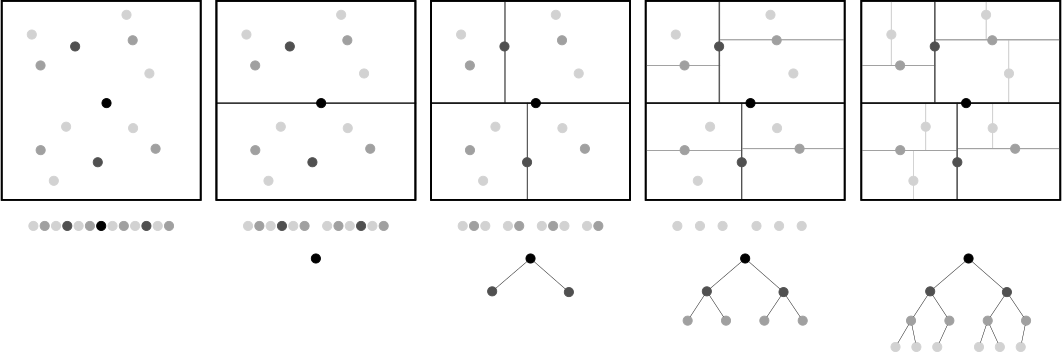
\includegraphics[width=\textwidth]{kdtree-tree}
  \caption[Konstruktion eines k-d-Baumes]{
    Rekursive Konstruktion eines k-d-Baumes: Die Punktmenge wird sortiert, der Median zum Baum hinzugefügt und seine Kinder aus den beiden Teilmengen per k-d-Baum-Konstruktion gewonnen.
    Der gewonnene Suchbaum ist effizient in Speicherplatz und Laufzeit der Suchoperationen.
  }
  \label{fig:kdtree}
\end{figure}

\begin{algorithm}
  \begin{algorithmic}
    \Input $points$ - Liste von Punkten
    \Input $k$ - Dimensionalität des Simulationsraumes
    \Result Root-Element eines vollständigen KD-Baumes aus diesen Punkten
    \State
    \Function{construct-kdtree}{$points, dim\gets0$}
    \State $n\gets$\Call{length}{points}
    \If{$n=0$}
    \State \Return null
    \Else
    \State \Call{sort}{$points, dim$} \Comment{Sortiert $points$ nach pos[$dim$]}
    \State $root\gets{}points\left[\lfloor\frac{n}{2}\rfloor\right]$
    \State $dim\gets(dim+1)\mod{k}$
    \State $root.left \gets$ \Call{construct-kdtree}{$points\left[0:\lfloor\frac{n}{2}\rfloor-1\right], dim$}
    \State $root.right \gets$ \Call{construct-kdtree}{$points\left[\lfloor\frac{n}{2}\rfloor+1:n-1\right], dim$}
    \State \Return $root$
    \EndIf
    \EndFunction
  \end{algorithmic}
  \caption[Konstruktion eines k-d-Baumes]{Rekursive Konstruktion eines k-d-Baumes (naive Implementierung)}
  \label{algo:kdtree-construction}
\end{algorithm}

Probleme von k-d-Bäumen zeigen sich bei der Suche nach einer Oberfläche einerseits und bei periodischen Räumen andererseits.

Die Oberfläche entlang einer Hauptachse lässt sich per Range Search mit anschließender Sortierung der Ergebnisse in \BigO{k\log{n^{1-\frac{1}{k}}}}\todo{REFERENZ!}{} ermitteln.
Möchte man jedoch das Auftreffen eines Precursors mit beliebiger Inklination ermitteln, kann man auf keine optimale Methode zurückgreifen.

Periodische Räume auf der anderen Seite brechen die Sucheigenschaften des k-d-Baumes, jedoch bloß am Rand der Struktur.
Nutzt man einen kleinen Suchbereich mit Radius $r$, der den Simulationsraum vollständig überlappt, so kann man die Periodizität vernachlässigen.
Andernfalls muss man entsprechend viele Suche in periodischen Bildern durchführen.
Die Modifikationsoperationen selbst bleiben unverändert.

Der größte Nachteil eines k-d-Baumes bleibt jedoch die Eigenschaft, beim Hinzufügen von Atomen beispielsweise entlang der z-Richtung stetig unbalancierter zu werden, wodurch Up\-date-Opera\-tionen auf dem gesamten Baum notwendig wären.
Diese sind mit der geringen Konstruktionszeit zwar vertretbar, allerdings unnötig in Hinblick auf andere Methoden, wie Octrees und Delaunay-Triangulationen.

\subsection{Delaunay-Triangulation}

\begin{figure}[bhpt]
  \centering
  \def\svgwidth{\textwidth}
  \input{img/delaunay.pdf_tex}
  \caption[Delaunay-Triangulation]{Beispiel der Konstruktion einer Delaunay-Triangulation (c) aus einer Punktwolke (a).
    Für jedes Simplex (hier 2d-Simplex, also Dreieck) muss das Delaunay-Kriterium eingehalten werden:
    Es dürfen sich keine weiteren Punkte im Umkreis des Simplices befinden (b).
  }
  \label{fig:delaunay}
\end{figure}

Eine alternative Partitionsmethode findet sich in Triangulationen.
Diese zerlegen den Raum nicht in Quader, sondern in k-dimensionale Simplexe, also geometrische Objekte voller Dimensionalität bei minimalen Punkten im jeweiligen Raum.
Anschaulich ergeben sich damit Dreiecke in zwei und Tetraeder in drei Dimensionen.
Diese Simplexe unterliegen besonderen Eigenschaften hinsichtlich der Punktmenge, jedoch möchte ich im Weiteren auf Delaunay-Triangulationen im Speziellen eingehen.

Delaunay-Triangulationen, so benannt nach ihrem Entdecker Boris Delaunay\todo{ref} besitzen besondere Eigenschaften, die sich als hilfreich in vielen algorithmischen Problemen zeigt.
So beinhaltet eine Delaunay-Triangulation eine Menge an Untergraphen, wie dem Nächstnachbargraph oder der Alphaform, die bei vielen Problemlösungen heran gezogen werden und auch hier von Interesse sein sollen.
Weiterhin ist sie dual zum Voronoi-Diagramm, was im Rahmen meiner Arbeit nicht weiter von Vorteil ist.
Die Haupteigenschaften einer Delaunay-Triangulation sind dabei Folgende:

\begin{itemize}
\item Jeder Punkt ist ein Eckpunkt mindestens eines Simplexes
\item Simplexe überschneiden sich nicht
\item Im Umkreis eines Simplexes befinden sich keine fremden Punkte
\item Die Vereinigung aller Simplexe ergibt die konvexe Hülle
\item Ein Punkt teilt sich mit seinem nächsten Nachbarn mindestens einen Simplex \\
  $\Leftrightarrow$ Nächstnachbargraph $\subset$ Delaunay-Triangulation
  %% \item Die Delaunay-Triangulation und das Voronoi-Diagramm über die selben Punkte sind dual\\
  %% $\Rightarrow$ Allgemeine Nachbarschaftssuche ist \BigO{k\log k}
\end{itemize}

Interessant werden sie aber nicht nur zur Speicherung von Atomen im Simulationsraum, sondern vor allem bei der Suche der Oberfläche und des Volumens sowie zur Konnektivitätsprüfung eines Systemes und somit im Rahmen der Auswertung von Punktwolken.
Dafür nutzt man eine Alpha-Form, die durch eine Untermenge der triangulierten Punktmenge definiert ist, die deren scheinbare Oberfläche bilden.
Es werden ebenso Oberflächenrauheiten und Dichten bis hin zu Nanoporen und Kristalldefekten abgebildet.
Mit wenig Mehraufwand ließen sich somit bei laufenden Simulationen diese Werte in-situ ermitteln und direkt einer Auswertung zuführen.
Andererseits ist die Oberfläche des Systemes zur Laufzeit bekannt und kann beispielsweise für Oberflächenreaktionen direkt genutzt werden.

\subsubsection{Algorithmen zur Konstruktion einer Delaunay-Triangulation}

Eine Delaunay-Triangulation lässt sich aus einer Punktmenge in \BigO{n\log n} konstruieren\todo{Algorithmus?}, wofür eine Vielzahl an Algorithmen zur Verfügung stehen. \todo{Referenz}
Diesen liegt das Delaunay-Kriterium zu Grunde:
Der Umkreis eines Simplices enthält nur seine eigenen Eckpunkte.
Ansonsten unterscheiden sie sich stark in Funktionsweise, Optimaler Laufzeit  und eventueller Parallelisierbarkeit.

\begin{itemize}
\item Flip-basierte Algorithmen (Local Improvement)\\
  Man startet mit einer beliebigen Triangulation, prüft den Umkreis aller Simplexe und führt gegebenenfalls den Flip-Algorithmus aus, der in Abbildung \ref{fig:delaunay-flip} vorgestellt wird.
  Diese Algorithmen konvergieren typischerweise in \BigO{n^2} und sind damit vergleichsweise langsam.

\item Scan-Algorithmus (Incremental Construction)\\
  Bei dieser Methode baut man schrittweise Simplexe auf, die das Delaunay-Kriterium erfüllen, ohne bestehende Simplexe löschen zu müssen.
  Man baut die Triangulation gewissermaßen \textit{von innen} auf.
  Durch viele Vergleiche und Sortierungen varieren typische asymptotische Laufzeiten zwischen \BigO{n\log{n}} und \BigO{n^2}.

\item Einfügungs-Algorithmen (Incremental Insertion)\\
  Sie sind das Gegenstück zu Scan-Algorithmen, insofern man hier die Triangulation \textit{von außen} aufbaut.
  Man erstellt einen beliebig großen Simplex, der die gesamte Punktmenge beinhaltet, und fügt nun schrittweise einzelne Punkte in die Triangulation ein.
  Der den neuen Punkt einschließende wird in mehrere Simplexe unterteilt, die anschließend bei auf das Delaunay-Kriterium überprüft und bei Bedarf geflippt werden.
  Mit ihnen erreicht man geringe Laufzeiten von \BigO{n\log{n} + n^{\lceil d/2 \rceil}}.

\item Divide-and-Conquer-Algorithmen\\
  Diese rekursiven Algorithmen ermöglichen durch effiziente Aufteilung des Problemes in zwei oder mehr Unterprobleme geringe Laufzeiten für viele Probleme, jedoch müssen dafür mehrere Probleme gelöst werden.
  Einerseits muss das Problem teilbar sein, was bei Punktmengen ohne weiteres möglich ist.
  Andererseits muss man die Lösungen der Teilprobleme zu einer Lösung des Gesamtproblemes zusammen gefügt werden.
  Bei Delaunay-Triangulationen gibt es verschiedene erfolgreiche Ansätze in zwei Dimensionen\todo{Referenzen}, die zu Laufzeiten nahe der für Divide and Conquer üblichen \BigO{n\log{n}} führen, jedoch stellen höhere Dimensionen diese Algorithmen vor Probleme.

  Cignoni et al.\cite{cignoni_1998} haben eine DeWall genannte\footnote{DeWall steht hier für Delaunay Wall Algorithm, so benannt nach den Wänden, an denen getrennt und wieder verknüpft wird} Methode gefunden, die eine zwar worst-case-Laufzeit von \BigO{n^{\lceil d/2 \rceil + 1}} ergibt, die sich jedoch nur in pathologischen Fällen zeigt.
  Nimmt man annähernde Gleichverteilungen an, die im vorliegenden Anwendungsfall gegeben sind, konvergiert dieser Algorithmus in drei Dimensionen subquadratisch und ist somit vergleichbar effizient.
  Es zeigt sich allerdings, dass er trotz der vermeintlich langen Laufzeit vor allem bei periodischen und periodisch erweiterten Systemen effizient arbeitet, da hier ohnehin Grenzflächen existieren, an denen Teiltriangulationen auf einander abgestimmt werden müssen.
  Andererseits ist das Parsivald-Modell ohnehin für parallele Platformen ausgelegt, so dass hier weitere Leistungssteigerungen zu erwarten sind.
  Ebenso eignet sich diese Methode zur Einbettung neu berechneter Würfel in die Struktur, wie es beim Parsivald-Modell nach jeder simulierten Reaktion vorkommt.

\item Höherdimensionale Einbettung\\
  Hier wird die Punktmenge in eine höhere Dimension transformiert, in der deren konvexe Hülle berechnet wird, die dann in den ursprünglichen Raum herunterprojiziert wird und darin eine zulässige Delaunay-Triangulation ergibt.
  In der Praxis ist dieser Algorithmus nicht weiter von Bedeutung, da Einfügungs-Algorithmen für allgemeine Fälle eine geringere Laufzeit erreichen.

\end{itemize}

\subsubsection{Flip-Algorithmus}

Viele dieser Algorithmen basieren auf dem \textbf{Flip-Verfahren}, mit dem invalide Simplexe in valide Simplexe überführt werden können.
Abbildung \ref{fig:delaunay-flip} stellt dar, wie man dabei den Simplex auf das Umkreis-Kriterium prüft und gegebenenfalls eine Grenzfläche zwischen zwei Simplexen auflöst und aus deren Punkten neue Simplexe erstellt, die das Delaunay-Kriterium erfüllen.
Anschließend führt man den selben Test mit deren Nachbarn durch.

\begin{figure}[bhpt]
  \captionsetup[subfigure]{singlelinecheck=false}{
    \def\subfigwidth{0.23\textwidth}
    \def\svgwidth{\textwidth}
    \begin{subfigure}[t]{\subfigwidth}
      \includegraphics[width=\textwidth]{delaunay-flip-a}
      \subcaption{Ausgangstriangulation}
      \label{fig:delaunay-flip-a}
    \end{subfigure}
    \hfill
    \begin{subfigure}[t]{\subfigwidth}
      \includegraphics[width=\textwidth]{delaunay-flip-b}
      \subcaption{Vereinigung invalider Simplexe}
      \label{fig:delaunay-flip-b}
    \end{subfigure}
    \hfill
    \begin{subfigure}[t]{\subfigwidth}
      \includegraphics[width=\textwidth]{delaunay-flip-c}
      \subcaption{Aufteilung in neue valide Simplexe}
      \label{fig:delaunay-flip-c}
    \end{subfigure}
    \hfill
    \begin{subfigure}[t]{\subfigwidth}
      \includegraphics[width=\textwidth]{delaunay-flip-d}
      \subcaption{Ergebnis}
      \label{fig:delaunay-flip-d}
    \end{subfigure}
  }
  \caption{
    Flip Algorithmus zur Aktualisierung einer Delaunay-Triangulation.
    Anschließend müssen Nachbar-Simplexe den selben Test durchlaufen.
    Die Flipping-Kaskade führt dabei höchstens \BigO{k\log{k}} Prüfungen aus, wenn man eine bestehende Delaunay-Triangulation aktualisieren möchte.
    $k$ steht hier für die Zahl der Simplexe eines Punktes.
  }
  \label{fig:delaunay-flip}
\end{figure}

\subsubsection{Nachbarschaftssuche}
Für die Nachbarschaftssuche eines Referenzpunktes werden die raumfüllenden Eigenschaften der Triangulation relevant.
Der notwendigerweise konvexe, sonst aber beliebige Suchbereich um den Referenzpunkt wird von Simplexen überdeckt, die in direkter oder indirekter Nachbarschaft des Punktes liegen.
Somit teilen sich alle Punkte innerhalb des Suchbereiches eine Kante eines Simplexes mit einem anderen Punkt im Suchbereich, sofern der Suchbereich hinreichend groß ist.
Ausgehend vom Referenzpunkt sucht man entlang aller Kanten nach Punkten, die innerhalb des Suchbereiches liegen, bis alle potentiellen Punkte überprüft wurden.
Diese Vorgehensweise ist in Algorithmus \ref{algo:delaunay-neigbors} ausführlich beschrieben.

\begin{algorithm}
  \centering
  \begin{algorithmic}
    \State Result = \{\}
    \State Queue = \{ P$_0$ : P$_0 \in$ Volume \}
    \While{Queue $\neq \emptyset$}
    \State Sei P $\in$ Queue
    \State Queue = Queue $\setminus$ \{ P \}
    \If{P $\in$ Volume}
    \State Result = Result $\cap$ \{ P \}
    \State Queue $\cap$ (Neighbors(P) $\setminus$ Result)
    \EndIf
    \EndWhile
  \end{algorithmic}
  \caption[Nachbarschaftssuche auf einer Delaunay-Triangulation]{Nachbarschaftssuche auf einer Delaunay-Triangulation.
    Ist der Suchraum konvex und hinreichend groß, lässt sich damit effizient nach Nachbarn eines bestimmten Punktes suchen.
  }
  \label{algo:delaunay-neighbors}
\end{algorithm}

\subsubsection{Alpha-Form}

Betrachtet man ausschließlich die Atome aller Simplexe, deren Umkreisradius oberhalb eines Grenzwertes $\alpha^{-1}$ liegt, so erhält man eine so genannte Alpha-Form (Alpha-Shape), wie in Abbildung \ref{fig:delaunay-alpha} dargestellt.
Diese umfasst neben den Punkten der konvexen Hülle ebenfalls je nach $\alpha$-Wert auch Poren und Dellen auf der Oberfläche sowie im Bulk, wobei Konnektivitätsinformationen aus der Delaunay-Triangulation gewonnen werden können.
Der algorithmische Mehraufwand zur Erstellung und Verwaltung dieser Informationen ist gegenüber der eigentlichen Delaunay-Triangulation vernachlässigbar\todo{Referenz}.
Aus diesem Grund bietet sich an, Oberflächensimulationen mit dem Parsivald-Modell mit Hilfe von Delaunay-Triangulationen zu verwalten, da die Oberflächeninformationen direkt in einen KMC-Algorithmus eingearbeitet werden können und somit auf separate Oberflächensuchen und -parametrisierungen verzichtet werden kann.

\begin{figure}[bhpt]
  \centering
  \captionsetup[subfigure]{singlelinecheck=false}{
    \def\subwidth{0.3\textwidth}
    \def\svgwidth{\textwidth}
    \begin{subfigure}[t]{\subwidth}
      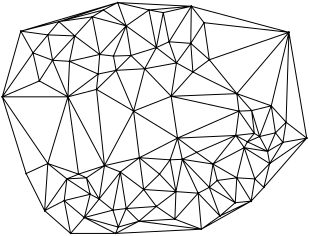
\includegraphics[width=\textwidth]{delaunay-alpha-a}
      \subcaption{Delaunay Triangulation}
      \label{fig:delaunay-alpha-a}
    \end{subfigure}
    \hfill
    \begin{subfigure}[t]{\subwidth}
      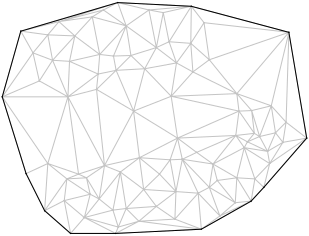
\includegraphics[width=\textwidth]{delaunay-alpha-b}
      \subcaption{Konvexe Hülle: Kanten mit nur einem Simplex}
      \label{fig:delaunay-alpha-b}
    \end{subfigure}
    \hfill
    \begin{subfigure}[t]{\subwidth}
      \includegraphics[width=\textwidth]{delaunay-alpha-c}
      \subcaption{Alpha-Form: Hülle nach Entfernung von Simplexen mit $\text{Umkreis} > \alpha$}
      \label{fig:delaunay-alpha-c}
    \end{subfigure}
  }
  \caption{Konstruktion einer Alpha-Form}
  \label{fig:delaunay-alpha}
\end{figure}
